\chapter{Theory}

This work showcases the use of \acp{pomdp} to model and solve decision making
problems in robotics with inherent uncertainty. In order to provide a baseline
for further discussions of specific application domains
(\cref{chap:applications}) we first introduce some of the throughout this work.
It should be noted that in the interest of conciseness we focus this
theoretical introduction on only the main tools use. Fundamental concepts of
statistical inference and tools like \textit{Monte Carlo Integration} are
assumed to be known. For a thorough discussion of these underlying concept the
reader may refer to \cite{kochenderfer2015decision, bertsekas2005dynamic, thrun2005probabilistic}.

In the following, we first introduce the theoretical framework of \acp{pomdp}
(\cref{sec:pomdp}). This section discusses modelling assumptions, structure
of solutions as well as theoretical properties of \acp{pomdp}. Thereafter,
\cref{sec:online-pomdp-solvers} describes two state-of-the-art online solution
methods for problems of this domain.

\section{Partially Observable Markov Decision Processes}\label{sec:pomdp}

The \acf{pomdp} is a principled mathematical formalism capable of representing
a broad range of sequential decision making problems under uncertainty. As the
name suggests, this framework is a generalization of the more popular \ac{mdp}
to the partially observable case. Thus, before proceeding with the full
complexity of a \ac{pomdp} let us first examine it's fully observable version.

\subsection{MDP}

\acp{mdp} are sequential decision making problems in which an agent takes
\vname{actions} $a$ that affect the \vname{state} $s$ of the environment and
receives \vname{rewards} $r$ based the state-transition and the action taken
\cite{kochenderfer2015decision, bertsekas2005dynamic}. The state evolves
according to a stochastic transition model $\tdist$ that and obeys the
Markov property. That is, future states are independent of past states given
the current state and action. By this means, \acp{mdp} allow to model outcome
uncertainty. As common in literature, we denote quantities at time time $t$
with an according subscript. When examining only a single step in a context
where time does not explicitly matter, we may also refer to states before and
after the transition as $s$ and $s'$ rather than $s_t$ and $s_{t+1}$.

Formally, an \ac{mdp} is fully characterized by the following quantities:

\begin{description}
  \item[State Space $\sspace$.] The set of all possible states.
  \item[Action Space $\aspace$.] The set of all possible actions.
  \item[Transition Model $\tdist$.] A model to represent the likelihood of
    each transition. This model provides $\tdist(s' \mid s, a)$, the
    probability of state $s'$ given that previously the environment was in
    state $s$ and the agent took action $a$.
  \item[Reward Function $\reward: \sspace \times \aspace \times
    \sspace \to \reals$.] A deterministic mapping that assigns
    a real-valued reward $r$ to each transition $(s, a, s')$ with finite transition
    probability, $\tdist(s' \mid s, a) > 0$.
  \item[Discount Factor $\gamma$.] A scalar that governs how rewards
    are discounted in the future.
\end{description}

The objective of the agent in the \ac{mdp} is to maximize the expected
cumulative rewards. Formally, this translates to finding a \vname{policy} $\pi:
\sspace \to \aspace$, that maps each encountered $s$ to an action $a
= \pi(s)$, such that following this policy maximizes the objective,

\begin{equation} \label{eq:objective}
    J(\pi) = E\left[\sum_{t=0}^\infty \gamma^t \reward(s_t, \pi(s_t), s_{t+1})\right] \text{.}
\end{equation}

An optimal solution to an \ac{mdp} can always be formulated as a deterministic
Markov policy, even though the reward that a policy achieves may be randomized
through $\tdist$. Consequently, there always exists a maximizer $\pi^*$ of
\cref{eq:objective}, where $\pi^*$ assigns a single action to every state.
Also, since the state obeys the Markov property, no additional information
beyond the current state at every time is necessary to maximize $J$
\cite{altmann1999constrained}.

\subsection{Partially Observable MDP}

A \acf{pomdp} is an \ac{mdp} where the agent cannot directly observe the state,
but instead at every time step $t$ receives an \vname{observation} $o_t$,
emission of the latent state $s_t$ and action $a_t$. By this means,
a \ac{pomdp} is able to encode state uncertainty in addition to the outcome
uncertainty present in the underlying \ac{mdp}.

Having introduced the properties of an \ac{mdp} in the previous section,
a generalization of this formalism to the partially observable case is obtained
by augmenting the 5-tuple $(\sspace, \aspace, \tdist, \reward,
\gamma)$ describing the underlying \ac{mdp} with the following quantities:

\begin{description}
  \item[Observation Space $\ospace$.] The set of all possible observations.
  \item[Observation Model $\odist$.] A model to represent the likelihood
    of each observation $o$ given the current state of the environment and the
    action taken at that time. Formally, this model provides the
    conditional probability $\odist(o \mid s, a)$ for each $(o, s, a) \in
    (\ospace \times \sspace \times \aspace)$.
\end{description}

The dynamic decision network representing the information structure for
a finite time horizon of a \ac{pomdp} is depicted in
\cref{fig:pomdp}.\todo{@zach is information structure the right word here? Or
is this only valid for game theory?} As evident from this figure, the decision
of the agent at time $t$ is informed by the sequence of all previous actions
and observations as well as some prior knowledge, $b_0$. In contrast to the
fully observable case where the policy is only a function of quantities at the
current time, the policy in a \ac{pomdp} maps each possible \vname{history},
${h_t = (b_0, a_0, o_1, a_1, \dots, a_{t-1}, o_t)}$ to an action, $a_t$.

\begin{figure}[htpb]
  \centering
  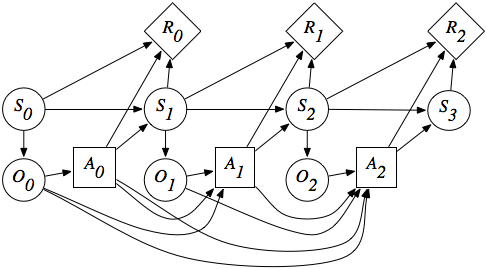
\includegraphics[width=.7\textwidth]{pomdp-dynamic-decision-network.png}
  \caption{The POMDP as a dynamic decision network. \todo[inline]{Replace with
  vector graphics and add initial information $b0$}}
  \label{fig:pomdp}
\end{figure}

In cases where this history can be compressed to a probability for every state
at time $t$, we will refer to this distribution as the \vname{belief},
$b_t(s)$. This belief is a sufficient statistic for optimal decision making.
Consequently, there exists a policy $\pi^*(b_t)$ only dependent on the belief
at the current time step, such that choosing ${a_t=\pi^*(b_t)}$ maximizes
\cref{eq:objective} subject to the constraints on the information pattern
imposed by the \ac{pomdp}, \cite{kaelbling1998planning,
kochenderfer2015decision}. Loosely speaking, $b_t$ preserves all relevant
information contained in the action-observation-history, $h_t$ necessary to
compute the optimal action. The belief is maintained by recursively performing
a Bayesian update,
\begin{equation} \label{eqn:update}
    b'(s') = \frac{\int_{s\in\sspace} \odist(o \mid s, a, s') \tdist(s' \mid s, a) b(s) \, ds}
    {\int_{s'\in\sspace} \int_{s\in\sspace} \odist(o \mid s, a, s') \tdist(s' \mid s, a) b(s) \, ds \, ds'} \text{.}
\end{equation}
with incoming observations, $o$. In the case of a discrete state space,
$\sspace$ integrals a to be replaced with sums. In cases where this update rule
is too complex to be evaluated analytically, Monte Carlo integration may be
used for approximate inference \cite{kochenderfer2015decision,
thrun2005probabilistic}.

Solutions to a \ac{pomdp} are Markov policies on belief states. That is, the
optimal policy $\pi^*(b(s)): \bspace \to \aspace$ selects action ${a =
\pi(b(s))}$ for each belief in the \vname{belief space}, $\bspace$ under the
objective of maximizing \cref{eq:objective}. Alternatively, when thinking of
this procedure in terms of action-observation-histories, the policy may be
envisioned as a conditional plan reasoning over the optimal action to take for
every possible sequence of actions and observations starting from the root
belief, $b_0$.\todo{visualization of conditional plan?} This perspective
reveals that the search space of possible policies rapidly grows with
increasing size of $\aspace$ and $\ospace$. In fact, it has been shown that
even in the case of finite-horizon problems \acp{pomdp} remain
PSPACE-complete. Hence, it is reasonable to assume to that no efficient general
algorithm for solving large problems of this class can be found
\cite{papadimitriou1987complexity}. However, recent research has made
significant progress on approximate solution methods, some of which we will use
in this work \cite{silver2010pomcp, somani2013despot, sunberg2018online}.

\todo[inline]{@zach: should this already contain some of the theoretical
advantages that one can expect?}

\section{Online POMDP Solvers}\label{sec:online-pomdp-solvers}

\todo[inline]{The solvers described here were chosen as they are state of the
art and show good performance over a range of problems. Point to Zach's paper
for solver performance comparison and DESPOT paper.}

\section{POMCPOW}

\todo[inline]{write:}
\begin{itemize}
  \item explain the basic idea of POMCPOW as Monte Carlo with DPW.
  \item is extension of POMCP with weighted particle beliefs.
\end{itemize}
\missingfigure{Pseudo Code with formal description in text.}

\missingfigure{graphical model of POMCP-Tree with weighted scenarios.}

\section{DESPOT}

\todo[inline]{write:}
\begin{itemize}
  \item formal, high-level idea of a DESPOT (idea of scenarios etc.)
  \item the search algorithm on a DESPOT with bounds
  \item explain the difference to POMCPOW (or Monte Carlo methods in general)
  \item point to literature for convergence guarantees
\end{itemize}

\missingfigure{DESPOT tree visualization}
\missingfigure{DESPOT algorithm Pseudo Code}

